\documentclass{ieeeaccess}

\usepackage{array}
\usepackage{cite}
\usepackage{amsmath,amssymb,amsfonts}
\usepackage{algorithmic}
\usepackage{graphicx}
\usepackage{textcomp}
\usepackage{multirow}
\usepackage[most]{tcolorbox}
\usepackage{xcolor}

\usepackage[most]{tcolorbox}
\usepackage{multicol}
\usetikzlibrary{positioning}

\newenvironment{Algorithm}[1][tbh]%
{\begin{myalgo}[#1]
\centering
\begin{minipage}{7.4cm}
\begin{algorithm}[H]}%
{\end{algorithm}
\end{minipage}
\end{myalgo}}


  \NewSpotColorSpace{PANTONE}
  \AddSpotColor{PANTONE} {PANTONE3015C} {PANTONE\SpotSpace 3015\SpotSpace C} {1 0.3 0 0.2}
  \SetPageColorSpace{PANTONE}%

\def\BibTeX{{\rm B\kern-.05em{\sc i\kern-.025em b}\kern-.08em
    T\kern-.1667em\lower.7ex\hbox{E}\kern-.125emX}}

\def\textsc#1{\textnormal{{\sc #1}}}%

\begin{document}

\title{\textsc{Daf-Cl}: A Robust Multimodal Emotion Classification Framework with Dynamic Adaptive Fusion and Contrastive Learning}

% \author{\uppercase{Saja~Taweel}\authorrefmark{1}, \uppercase{Mohammad~J.~Abdel-Rahman}\authorrefmark{1}\IEEEmembership{Senior Member,~IEEE}, \uppercase{Noor Alawi}\authorrefmark{1}, \uppercase{Jude Daghlas}\authorrefmark{1}, and \uppercase{Ahmad Ghunaim}\authorrefmark{1}
% }

\author{\uppercase{}\authorrefmark{1},  \uppercase{}\authorrefmark{1}, and \uppercase{}\authorrefmark{1}
}

% \address[1]{Data Science Department, Princess Sumaya University for Technology, Amman 11941, Jordan}
%\address[2]{Electrical and Computer Engineering Department, Virginia Tech, Blacksburg, VA 24061 USA}


\markboth
{S.~Taweel \headeretal: \textsc{DAF-CL}: A Robust Multimodal Emotion Classification Framework with Dynamic Audio-Text Fusion and Contrastive Learning}
{S.~Taweel \headeretal: \textsc{DAF-CL}: A Robust Multimodal Emotion Classification Framework with Dynamic Audio-Text Fusion and Contrastive Learning}

\corresp{Corresponding author:  (e-mail: ).}


\begin{abstract}

\end{abstract}


\begin{keywords}

\end{keywords}

\titlepgskip=-15pt

\maketitle
\def\textsc#1{\textnormal{{\sc #1}}}%

\section{Introduction}\label{sec:introduction}

\IEEEPARstart{E}{motion} plays a crucial role in human life, influencing decision-making processes and interpersonal interactions~\cite{COWIE20035}. With the rapid advancement of technology and the increasing integration of artificial intelligence into everyday tasks, there is a growing need to develop AI systems capable of understanding and responding to human emotions effectively~\cite{Venkataramanan2019}. In particular, intelligent assistants and conversational agents are expected to recognize emotional tone and generate responses that align with users’ affective states. However, relying solely on textual input is often insufficient, as human emotions are subtle, overlapping, and highly context-dependent, making them difficult to accurately capture using unimodal signals~\cite{PAYALA2026}. Furthermore, external factors such as background noise, variations in speaker tone, and environmental conditions introduce additional challenges for emotion recognition systems~\cite{PAYALA2026}. As a result, multimodal approaches that combine text and speech have gained attention due to their ability to capture complementary emotional cues from both linguistic and paralinguistic information. While visual signals, such as facial expressions, can further enhance emotion recognition performance, their practical adoption remains limited due to challenges in large-scale data collection, annotation, and real-world deployment constraints, including privacy concerns and user preferences~\cite{Lian2023}. In many real-world applications, users are more inclined to provide audio rather than video input, making audio–text multimodal systems a more feasible and scalable solution.

Emotion recognition has attracted increasing research attention in recent years, leading to significant advancements in both unimodal and multimodal learning frameworks. Early studies primarily focused on unimodal emotion recognition using either textual information\cite{Cortiz2022, Batbaatar2019, Han2023} or speech signals through handcrafted acoustic features\cite{Mustaqeem2020, Venkataramanan2019, Novais2023} and, more recently, self-supervised learned speech representations\cite{Atmaja2022, Yingzhi2021}. Although these approaches achieved promising performance, relying on a single modality often limits the ability of the model to capture the complete emotional context. To overcome these limitations, recent research has increasingly shifted toward multimodal emotion recognition by integrating complementary information from speech and text modalities. Existing multimodal approaches employ various fusion strategies, including feature interaction methods\cite{Koudounas2026, Chen2020, Chudasama2022, Dikbiyik2025, ISLAM2026, Kakuba2023}, cross-modal attention mechanisms\cite{Krishna2020}, knowledge distillation frameworks\cite{KIM2026}, and ensemble-based approaches that combine independently learned predictions or representations from different modalities\cite{PAYALA2026, Sebastian2019}. More recently, contrastive learning has emerged as an effective paradigm for multimodal representation learning. Existing contrastive multimodal approaches can generally be categorized into cross-modal alignment methods\cite{qian2022}, fusion-integrated contrastive learning frameworks \cite{Shi2024, Li2025, Kim2023}, and pretraining-based contrastive approaches\cite{Jing2026, Nguyen2024}.

Several studies have demonstrated the effectiveness of multimodal learning and contrastive objectives for emotion recognition. For example, the ablation study presented in\cite{Shi2024} showed that multimodal fusion significantly outperformed unimodal approaches on both the IEMOCAP and MELD datasets, achieving approximately 18\% improvement compared to speech-only models and around 4\% improvement compared to text-only models. Similarly, \cite{qian2022} reported that incorporating cross-modal contrastive alignment improved weighted accuracy on the IEMOCAP dataset by 1.44\%. In addition,\cite{Li2025} demonstrated that integrating label-aware contrastive learning within multimodal fusion increased the weighted average F1-score on the MELD dataset by approximately 4\%. These findings collectively highlight the effectiveness of combining multimodal learning with contrastive representation objectives for emotion recognition tasks.

Despite these advances, several challenges remain insufficiently addressed. Existing methods still struggle to achieve robust generalization across different datasets, speakers, and linguistic distributions, while many fusion strategies rely on static interactions that fail to adaptively model the varying reliability and importance of modalities across conversational contexts. Furthermore, current contrastive learning approaches often focus on either cross-modal alignment or discriminative representation learning independently, limiting their ability to jointly optimize semantic consistency and emotional separability within multimodal representations. To address these limitations, we propose a unified multimodal framework that integrates speech and text through a dynamic utterance-level fusion mechanism combined with structured cross-modal contrastive learning.

Specifically, the proposed framework introduces a chunk-based audio modeling strategy in which each utterance is segmented into overlapping temporal chunks to better capture fine-grained variations in emotional expression. Supervised contrastive learning is applied at the chunk level to enhance intra-class compactness and inter-class separability within the audio representation space. To further improve robustness, a confidence-aware aggregation mechanism is employed to weight chunk-level representations according to their reliability, producing a more stable utterance-level embedding. In parallel, a cross-modal contrastive objective aligns audio and text representations within a shared embedding space, improving inter-modal consistency. By jointly optimizing dynamic fusion, chunk-level supervised contrastive learning, cross-modal alignment, and confidence-aware aggregation, the proposed framework achieves improved generalization and provides a robust and discriminative solution for multimodal emotion recognition across diverse conditions.

\subsection*{Main Contributions:}

\begin{itemize}
\item We propose \textsc{Daf-Cl}, a unified multimodal emotion recognition framework that jointly learns dynamic audio–text fusion and cross-modal representation alignment. The proposed approach adaptively balances modality contributions at the utterance level, enabling robust performance under varying modality reliability and noise conditions.
\item We introduce a chunk-based audio representation learning strategy combined with supervised contrastive learning to capture fine-grained temporal variations in speech while enhancing intra-class compactness and inter-class separability.
\item We design a confidence-aware aggregation mechanism that adaptively weights chunk-level representations according to their reliability, producing more stable and robust utterance-level representations.
\item We formulate a unified multi-objective optimization framework that jointly integrates classification loss, cross-modal contrastive alignment, and supervised contrastive learning to enable end-to-end learning of discriminative and aligned multimodal representations.
\item We conduct extensive experiments and ablation studies across multiple datasets and cross-lingual settings, demonstrating the robustness and generalization capability of the proposed framework under diverse conditions.
\end{itemize}

\subsection*{Paper Organization:} The rest of the paper is organized as follows. In Section~\ref{sec:related work}, we review previous work related to our paper. In Section. In Section~\ref{sec:Model 1}, we develop our framework, \textsc{Daf-Cl}. Then, in Section~\ref{sec:performance evaluation}, . Finally, the main conclusions of this paper are summarized in Section~\ref{sec:Conclusion}.




\section{Related Work}\label{sec:related work}

Emotion recognition has evolved significantly over recent years, progressing from traditional unimodal approaches toward more advanced multimodal and contrastive learning frameworks. Early research primarily focused on unimodal emotion recognition using either textual or acoustic information independently\cite{Cortiz2022, Batbaatar2019, Han2023, Mustaqeem2020, Venkataramanan2019, Novais2023, Atmaja2022, Yingzhi2021}. Although these approaches demonstrated promising performance, relying on a single modality often limits the model’s ability to capture the full emotional context. Consequently, later studies shifted toward multimodal frameworks that integrate complementary information from different modalities through various fusion strategies\cite{Koudounas2026, Chen2020, Chudasama2022, Dikbiyik2025, ISLAM2026, Kakuba2023, Krishna2020, KIM2026, PAYALA2026, Sebastian2019}. More recently, contrastive learning has emerged as an effective paradigm for improving multimodal representation learning by enhancing cross-modal alignment and increasing intra-class discriminability\cite{qian2022, Kim2023, Shi2024, Li2025, Jing2026, Nguyen2024}. Figure \ref{fig:RW-taxonomy} summarizes the main directions in emotion recognition research and highlights representative studies within each category.

\begin{figure*}
	\centering
	\begin{tikzpicture}[
		scale=1, 
		transform shape, 
		level 1/.style={sibling distance=6cm, level distance=2cm, text width=3.5cm}, 
		level 2/.style={sibling distance=3.5cm, level distance=1.5cm, text width=3cm},
		every node/.style={draw, align=center, rectangle, rounded corners, text centered, minimum height=1cm, inner sep = 12pt},
		every child/.style={anchor=north},
		edge from parent/.style={draw, thick, ->, >=stealth},
		node distance=2.25cm,
		text width=2.25cm,
		text height= 0.01cm,
		]
		
		
		% define root %
		\node[root][fill=gray!25!white, text width=5cm] {\textbf{Emotion Classification}}
		% Level-1 children %
		child {node[level-2][fill=green!25!white] (c1) {\textbf{Unimodal}}
			child {node[fill=green!10!white, text width=2.25cm, text height = 0.01cm](c11) {\textbf{Speech-based \newline }}}
			child {node[fill=green!10!white, text width=2.25cm, text height = 0.01cm](c12) {\textbf{Text-based} \\ \cite{Cortiz2022, Batbaatar2019, Han2023}}}
		}
		child {node[level-2][fill=pink!50!white] (c2) {\textbf{Multimodal}}}   
		child {node[level-2][fill=cyan!25!white] (c3) {\textbf{Multimodal \& Contrastive Learning}}};
		\begin{scope}
			% For Category 1 children %
			\node [below of = c11, xshift=15pt][fill=green!10!white] (c111) {\textbf{Handcrafted Features} \\ \cite{Mustaqeem2020, Venkataramanan2019, Novais2023}};
			\node [below of = c111][fill=green!10!white] (c112) {\textbf{Learned Representations} \\ \cite{Atmaja2022, Yingzhi2021}};
			% For Category 2 children %
			\node [below of = c2, xshift=15pt][fill=pink!20!white] (c21) {\textbf{Feature Interaction} \\ \cite{Koudounas2026, Chen2020, Chudasama2022, Dikbiyik2025, ISLAM2026, Kakuba2023}};
			\node [below of = c21][fill=pink!20!white] (c22) {\textbf{Attention-based}  \\ \cite{Krishna2020}};
			\node [below of = c22][fill=pink!20!white] (c23) {\textbf{Knowledge Distillation} \\ \cite{KIM2026}};
			\node [below of = c23][fill=pink!20!white] (c24) {\textbf{Ensemble-based} \\ \cite{PAYALA2026, Sebastian2019}};
			
			% For Category 3 children %
			\node [below of = c3, xshift=15pt][fill=cyan!10!white] (c31) {\textbf{Cross-modal Alignment} \\ \cite{qian2022}};
			\node [below of = c31][fill=cyan!10!white] (c32) {\textbf{Fusion-Integrated} \\ \cite{Shi2024, Li2025, Kim2023}};
			\node [below of = c32][fill=cyan!10!white] (c33) {\textbf{Pretraining} \\ \cite{Jing2026, Nguyen2024}};
			\node [below of = c33][fill=yellow!20!white] (c34) {\textbf{{Structured Cross-modal SupCL \\( \textsc{Daf-Cl})}}};
			
		\end{scope}
		
		
		% Draw arrows from level-1 to it's children %
		\foreach \value in {111, 112}
		\draw[->] (c11.194) |- (c\value.west);
		\foreach \value in {1,...,4}
		\draw[->] (c2.194) |- (c2\value.west);
		
		\foreach \value in {1,...,4}
		\draw[->] (c3.194) |- (c3\value.west);
		
	\end{tikzpicture}
	\caption{Taxonomy of Emotion Recognition: From Unimodal to Multimodal Contrastive Learning.}
	\label{fig:RW-taxonomy}
\end{figure*}


In text-based emotion recognition, transformer architectures have achieved strong performance in modeling contextual semantics and linguistic dependencies\cite{Cortiz2022}. However, semantic understanding alone is often insufficient for accurately capturing subtle emotional cues embedded within text. To address this limitation, several studies proposed ensemble-based approaches that separately learn semantic and emotional representations before combining them for final classification\cite{Batbaatar2019}. Building upon this idea, subsequent research introduced attention mechanisms to better emphasize emotionally relevant contextual information, leading to improved feature representation and classification performance\cite{Han2023}.

For speech-based emotion recognition, early approaches mainly relied on handcrafted acoustic features due to their structured and interpretable nature. These features have been widely used in both traditional machine learning and deep learning frameworks. Some studies transformed handcrafted features into two-dimensional representations to exploit the representational capabilities of visual models\cite{Mustaqeem2020, Venkataramanan2019}, while others directly processed one-dimensional acoustic feature vectors using ensemble learning and conventional classification models\cite{Novais2023}. Despite their effectiveness, handcrafted features remain limited in their ability to capture high-level emotional representations.
To overcome these limitations, recent research has increasingly adopted self-supervised learning (SSL) for speech representation learning. Instead of relying on manually designed acoustic descriptors, SSL models learn generalized and transferable representations directly from large-scale unlabeled speech data. Comparative studies have demonstrated the superiority of these learned representations over traditional handcrafted features across emotion recognition tasks\cite{Atmaja2022}. Furthermore, several works investigated different adaptation strategies, including full and partial fine-tuning, to better exploit pretrained speech representations for downstream emotional understanding\cite{Yingzhi2021}.

The transition from unimodal to multimodal emotion recognition was primarily motivated by the limitation of relying on a single modality to capture the complete emotional context. Consequently, recent research has increasingly focused on integrating complementary information from multiple modalities, particularly speech and text, through different fusion strategies. Existing multimodal approaches can generally be categorized into feature interaction, attention-based fusion, knowledge distillation, and ensemble-based methods.

A considerable portion of prior work focuses on feature interaction mechanisms, where modalities are jointly fused to enhance representation learning. Some studies emphasize one modality more than the other during the interaction process. For instance,\cite{Koudounas2026} refines textual representations using acoustic context, where audio information is utilized to disambiguate lexically neutral or ambiguous text through a multi-head attention fusion mechanism. In this framework, acoustic features serve as the keys and values, while textual representations form the query. Other approaches adopt a hybrid strategy by training independent models for each modality alongside an additional multimodal fusion model, followed by combining their predictions using ensemble learning\cite{Chen2020}. Furthermore, several studies incorporate intermediate fusion stages between modalities before the final classification layers to strengthen multimodal representation learning\cite{Chudasama2022, Dikbiyik2025}.

Beyond speech and text, some studies extend multimodal emotion recognition by incorporating the visual modality \cite{Chudasama2022, ISLAM2026}. These approaches extract visual representations using deep visual feature extraction techniques and subsequently integrate them with speech and textual information. For example,\cite{ISLAM2026} combines multiple handcrafted acoustic features before performing multimodal fusion with visual representations. Similarly,\cite{Kakuba2023} demonstrates that directly learning from raw speech and textual inputs can outperform traditional handcrafted feature extraction pipelines. Their framework combines CNNs, BiLSTM networks, self-attention, and multi-head attention modules for each modality independently, while employing multi-stage fusion strategies at different representation levels. Specifically, the model first fuses convolutional representations, followed by fusion after the self-attention BiLSTM layers, before aggregating all representations using a transformer encoder for final emotion classification.

Although attention mechanisms have been introduced in several multimodal frameworks, many studies still primarily rely on feature interaction as the core fusion philosophy. In contrast, attention-based approaches explicitly model the alignment between modalities through cross-modal attention mechanisms. For example,\cite{Krishna2020} employs cross-modal attention to enhance the interaction between textual and acoustic representations for emotion recognition. The framework utilizes 1D convolutional neural networks for feature extraction, while the cross-modal attention module enables the model to focus on emotionally salient information across modalities.

Other research directions focus on improving multimodal representation learning through knowledge distillation strategies. In \cite{KIM2026}, a dual distillation framework is proposed that combines both self-distillation and cross-modal distillation for multimodal emotion recognition in conversational settings. The self-distillation module enhances intra-modal feature representations by transferring knowledge within the same modality, while the cross-modal distillation module aligns complementary emotional information between speech and text modalities, resulting in more robust and discriminative multimodal representations.

In contrast to interaction-based methods, some approaches focus on combining independently learned predictions or representations from different modalities without performing deep cross-modal interaction during feature learning. These methods are generally categorized as ensemble-based fusion approaches \cite{PAYALA2026, Sebastian2019}. For instance,\cite{Sebastian2019} proposes an ensemble fusion framework optimized using the Aquila optimizer, where modalities are processed separately and their outputs are aggregated during the final decision stage. Similarly, \cite{PAYALA2026} independently learns audio and textual representations before combining their predictions for final emotion classification, without employing explicit cross-modal interaction mechanisms.

With the rapid advancement of self-supervised and contrastive learning, recent studies have increasingly incorporated contrastive objectives into multimodal emotion recognition frameworks. Existing approaches can generally be categorized into three main directions: cross-modal alignment, fusion-integrated contrastive learning, and pretraining-based methods.

Some studies focus primarily on aligning representations from different modalities through contrastive objectives, commonly referred to as cross-modal alignment methods. For example,\cite{qian2022} applies contrastive regularization between speech and text representations before multimodal fusion. In this framework, audio signals are first converted into Mel-spectrograms and processed using a CNN, while textual features are extracted using GloVe embeddings followed by an LSTM encoder. The learned representations are then passed through a discriminator that maximizes the similarity between paired audio-text embeddings while separating them from negative samples, thereby improving cross-modal representation consistency prior to fusion.

Another line of research integrates discriminative objectives during or after multimodal fusion, which can be categorized as fusion-integrated contrastive learning. In\cite{Kim2023}, the framework first performs multimodal fusion using a crossmodal transformer with focus-attention, enabling speech and text representations to interact and exchange contextual information. The fused representation is subsequently refined using a metric learning objective that enhances the separation between emotional classes within the embedding space. Similarly,\cite{Shi2024} also applies a discriminative objective after multimodal fusion; however, the underlying learning objective differs from\cite{Kim2023}. While\cite{Kim2023} mainly employs metric learning to optimize embedding distances and improve the geometric structure of emotional representations,\cite{Shi2024} explicitly encourages intra-class compactness and inter-class separability by pulling samples from the same emotion class closer while pushing different emotional classes farther apart. Extending this direction,\cite{Li2025} proposes a multilayer interaction framework that progressively exchanges information across multimodal representations to improve emotional feature learning. Unlike methods that apply contrastive learning only after the final fusion stage, MIMCL tightly integrates contrastive objectives within intermediate interaction modules, enabling iterative refinement of multimodal representations and improving emotional discriminability across multiple feature levels.

In contrast, other studies mainly employ contrastive learning during the pretraining stage to learn more generalized multimodal representations. For instance,\cite{Jing2026} introduces a contrastive language-audio pretraining framework for affective computing that aligns speech and textual representations using soft-target contrastive learning. Unlike conventional hard-label contrastive objectives, the proposed method leverages soft targets to capture nuanced emotional relationships between samples, resulting in more robust multimodal representations and improved downstream emotion recognition performance. Similarly,\cite{Nguyen2024} proposes a contrastive language-audio alignment framework that combines pretrained HuBERT speech representations with self-alignment learning to enhance emotional representation quality. Although multimodal contrastive learning is employed during pretraining, the downstream emotion recognition stage primarily relies on the enhanced speech representations, demonstrating the effectiveness of cross-modal pretraining for speech emotion understanding.

Our research addresses an important gap in the existing literature by introducing a Dynamic Adaptive Fusion with Contrastive Learning (\textsc{Daf-Cl}) framework that jointly integrates dynamic cross-modal fusion and structured supervised contrastive learning within a unified optimization framework. The proposed approach aims to address several limitations that remain insufficiently explored in current emotion recognition methods. Although recent multimodal contrastive learning approaches have demonstrated promising performance, existing methods still struggle to effectively model semantic alignment, adaptive multimodal interaction, and discriminative emotional representation learning simultaneously.

One major limitation of unimodal approaches is their restricted ability to capture complementary emotional information available across different modalities\cite{Cortiz2022, Batbaatar2019, Han2023, Mustaqeem2020, Venkataramanan2019, Novais2023, Atmaja2022, Yingzhi2021}. Consequently, multimodal emotion recognition has emerged as a promising direction; however, many existing multimodal frameworks still suffer from insufficient semantic alignment between heterogeneous modalities. For example, in\cite{Koudounas2026}, the framework primarily relies on textual representations while utilizing speech only to disambiguate lexically neutral or ambiguous text. Similarly, methods such as\cite{PAYALA2026, Dikbiyik2025} and\cite{ISLAM2026} mainly employ intermediate fusion strategies without explicitly ensuring optimal interaction and alignment between modalities.

Moreover, several existing multimodal approaches rely on static fusion mechanisms, which may inadequately model the varying contribution and importance of modalities across different emotional contexts \cite{Chen2020, Dikbiyik2025}, and \cite{Sebastian2019}. In realistic conversational settings, the emotional significance of speech and text may dynamically vary across utterances, making static fusion strategies less effective for robust emotion understanding.

Although contrastive learning has recently gained significant attention in multimodal emotion recognition, existing approaches often focus on either cross-modal alignment or class-level discrimination independently rather than jointly optimizing both objectives \cite{qian2022, Kim2023, Shi2024}. Furthermore, several studies apply contrastive objectives only after the final fusion stage, limiting progressive interaction refinement and multimodal representation learning throughout the network\cite{Kim2023, Shi2024, Li2025}. On the other hand, pretraining-based approaches improve representation quality during the alignment stage but often fail to fully exploit multimodal interaction during downstream emotion classification tasks \cite{Jing2026} and \cite{Nguyen2024}.

Another important limitation lies in the generalization capability of existing methods. Many studies primarily evaluate their frameworks on a limited number of benchmark datasets, particularly IEMOCAP and RAVDESS, without extensively investigating model robustness across different speakers, domains, and data distributions\cite{Nguyen2024, Venkataramanan2019, Chen2020,Dikbiyik2025} and\cite{Krishna2020, KIM2026, Sebastian2019, qian2022, Kim2023, Shi2024, Li2025}. As a result, the real-world generalizability of these models remains insufficiently explored.

To address these limitations, we propose the \textsc{Daf-Cl} framework, which combines dynamic adaptive multimodal fusion with structured supervised contrastive learning to jointly enhance cross-modal semantic alignment and emotional discriminability. The proposed framework is designed to enable more effective multimodal interaction, adaptive modality weighting, and improved generalization across diverse emotional contexts and data distributions, providing a scalable and robust solution for multimodal emotion recognition.





% \section{System Model and Problem Statement}\label{sec:system model and problem statement}

% \input{System Model and Problem Statement}



\section{\textsc{DAF-CL} Framework}\label{sec:Model 1}

In this section, we present the proposed \textbf{Dynamic Adaptive Fusion with Contrastive Learning (\textsc{Daf-Cl})} framework for multimodal emotion recognition. Given a multimodal utterance set denoted by ($\mathcal{D}$), the framework jointly models textual and acoustic information, represented as:

\begin{equation}
	\mathcal{D} = \{(t_i, u_i, y_i)\}_{i=1}^{N}
\end{equation}

where \(t_i\) and \(u_i\) denote the textual and
speech utterances of the \(i^{th}\) sample,
respectively, \(y_i\) represents the corresponding
emotion label, and \(N\) is the total number of
utterances in the dataset.

The proposed \textsc{Daf-Cl} framework consists of three major components. First, a structured supervised contrastive learning module is applied to overlapping speech chunks to enhance intra-class compactness and inter-class separability within the acoustic representation space. Second, a dynamic confidence-aware audio-text fusion mechanism is introduced to adaptively integrate multimodal information according to the contextual reliability of each modality. Third, a cross-modal contrastive alignment module is employed to improve semantic consistency between speech and textual representations by aligning heterogeneous modality embeddings within a shared representation space.

To jointly optimize these components, the framework is trained using a multi-objective learning strategy that combines supervised contrastive loss, cross-modal alignment loss, and emotion classification loss. The overall architecture is illustrated in Figure \ref{fig:model}. The following subsections describe each component in detail.
\begin{figure*}
	\centering
	\includegraphics[width=1\linewidth]{"modeldevelop}
	\caption{Framework development of the \textsc{Daf-Cl} model.}
	\label{fig:model}
\end{figure*}



\subsection{Audio Representation Learning}
Given an input speech utterance waveform $u_i$, we segment the signal into overlapping, fixed-length chunks to capture local emotional variations while maintaining a consistent input size for the downstream models. The main notations used throughout this subsection are summarized in Table \ref{tab:table0}.

\begin{table}[ht]
	\centering
	\caption{Notation summary for audio representation learning}
	\label{tab:table0}
	\begin{tabular}{|p{0.18\columnwidth} | p{0.72\columnwidth}|}
		\hline
		\textbf{Notation} & \textbf{Description} \\
		\hline
		\hline
		$M$ & Number of chunks per utterance \\
		\hline
		$c$ & Chunk duration in seconds \\
		\hline
		$f_s$ & Audio sampling rate \\
		\hline
		$\rho$ & Overlap ratio ($\rho \in [0, 1)$) \\
		\hline
		$\mathbf{X}_a^{(i,m)}$ & Extracted acoustic features for chunk $m$ of utterance $i$ \\
		\hline
		$L$ & Total number of WavLM Transformer layers \\
		\hline
		$\mathbf{H}_i^{(l, m)}$ & Hidden representation of chunk $m$ at layer $l$, $\mathbf{H}_i^{(l, m)} \in \mathbb{R}^{T_m \times d}$ \\
		\hline
		$T_m$ & Temporal frame length of chunk $m$ in the latent space \\ 
		\hline
		$d$ & Feature embedding dimension \\
		\hline
		$w_l$ & Trainable importance weight assigned to layer $l$ \\
		\hline
		$\omega_l$ & Softmax-normalized layer importance weight \\
		\hline
	\end{tabular}
\end{table}

The corresponding chunk length ($L_c$) and hop size ($L_h$) in terms of samples are defined as: 
\begin{equation}
	L_c = \lfloor c \cdot f_s \rfloor, \quad L_h = \lfloor L_c (1-\rho) \rfloor.
\end{equation}

The segmentation is performed using a sliding-window approach. The $m$-th chunk ($m \in \{1, \dots, M\}$) of the utterance waveform is extracted as:
\begin{equation}
	u_i^{(m)} = u_i[m L_h : m L_h + L_c].
\end{equation}
For utterances shorter than $L_c$, a single chunk is produced and zero-padded to match the fixed length $L_c$. For longer utterances, the window strides by $L_h$, and the final segment is padded if necessary. This strategy ensures fixed-length, overlap-aware acoustic segmentation.

Each chunk $u_i^{(m)}$ is processed by a pretrained WavLM to extract hierarchical acoustic features across multiple Transformer layers. To preserve the general acoustic knowledge learned during self-supervised pretraining while adapting to downstream emotion dynamics, the lower layers of WavLM are frozen, whereas the higher layers are fine-tuned. 

Unlike conventional approaches that rely solely on the final layer representation, the proposed framework introduces a trainable layer fusion mechanism to adaptively aggregate information across all $L$ layers. We define a vector of trainable layer weights:
\begin{equation}
	\mathbf{w} = [w_1, w_2, \dots, w_L],
\end{equation}
which are normalized via a softmax function to produce the layer-wise attention scores:
\begin{equation}
	\omega_l = \frac{\exp(w_l)}{\sum_{k=1}^{L}\exp(w_k)}.
\end{equation}
The layer-fused representation for chunk $m$ of utterance $i$ is then computed as:
\begin{equation}
	\mathbf{H}_{\text{fused}}^{(i,m)} = \sum_{l=1}^{L} \omega_l \mathbf{H}_i^{(l, m)}.
\end{equation}
This adaptive fusion mechanism enables the model to selectively emphasize specific Transformer layers that capture emotionally discriminative acoustic cues at different abstraction levels. 

To model the localized temporal dependencies within each chunk, the fused representation is passed through a vanilla Transformer encoder layer:
\begin{equation}
	\widetilde{\mathbf{H}}^{(i,m)} = \text{TransformerEncoder}(\mathbf{H}_{\text{fused}}^{(i,m)}).
\end{equation}
The frame-level representations are subsequently aggregated into a fixed-dimensional chunk embedding $\mathbf{z}_i^{(m)} \in \mathbb{R}^d$ using mean pooling across the temporal dimension:
\begin{equation}
	\mathbf{z}_i^{(m)} = \frac{1}{T_m}\sum_{t=1}^{T_m}\widetilde{\mathbf{H}}_{t}^{(i,m)},
\end{equation}
where $\widetilde{\mathbf{H}}_{t}^{(i,m)}$ denotes the $t$-th temporal frame of the encoded chunk.

Since different speech segments contribute unequally to the underlying emotional state, an adaptive reliability assessment mechanism is introduced. First, an emotional saliency score $\alpha_i^{(m)}$ is computed to estimate the emotional relevance of the chunk:
\begin{equation}
	\alpha_i^{(m)} = \sigma(\mathbf{W}_a \mathbf{z}_i^{(m)} + \mathbf{b}_a),
\end{equation}
where $\sigma(\cdot)$ is the sigmoid activation function, and $\mathbf{W}_a \in \mathbb{R}^{1 \times d}$ and $\mathbf{b}_a \in \mathbb{R}^1$ are learnable parameters.

Each chunk embedding is passed through the audio classification head $f_{\text{audio}}(\cdot)$ to compute the chunk-level emotion prediction logits $\mathbf{\ell}_i^{(m)}$:
\begin{equation}
	\mathbf{\ell}_i^{(m)} = f_{\text{audio}}(\mathbf{z}_i^{(m)}).
\end{equation}

The model's local prediction confidence is defined using the maximum softmax probability over the predicted logits:
\begin{equation}
	c_i^{(m)} = \max_{k \in \mathcal{Y}} \text{softmax}(\mathbf{\ell}_i^{(m)})_k,
\end{equation}
where $\mathcal{Y}$ denotes the set of emotion classes. 

The final chunk importance weight $\gamma_i^{(m)}$ scales its emotional saliency by its predictive confidence, acting as a gating mechanism for decision-level fusion:
\begin{equation}
	\gamma_i^{(m)} = \alpha_i^{(m)} \cdot c_i^{(m)}.
\end{equation}

Finally, the utterance-level decision vector $\mathbf{\ell}_i$ is achieved via a weight-normalized decision fusion step across all acoustic segments:
\begin{equation}
	\mathbf{\ell}_i^{\text{audio}} = \frac{\sum_{m=1}^{M} \gamma_i^{(m)} \mathbf{\ell}_i^{(m)}}{\sum_{m=1}^{M} \gamma_i^{(m)} + \epsilon},
\end{equation}
where $\epsilon > 0$ is a small constant preventing numerical instability. This decision-level fusion mechanism adaptively emphasizes predictions from emotionally clear speech regions while suppressing the influence of ambiguous or noisy chunks on the final utterance classification. 


\subsection{Text Representation Learning}
Given the text transcription associated with the $i$-th utterance, denoted by $t_i$, the framework leverages a pretrained RoBERTa encoder to capture semantic and contextual dependencies across the word tokens.

Following standard practice in RoBERTa-based language models, the contextual hidden vector corresponding to the special start-of-sentence token ($\texttt{<s>}$) is adopted as the utterance-level textual embedding:
\begin{equation}
	\mathbf{z}_i^{\text{text}} = \mathbf{h}_{i,\texttt{<s>}}
\end{equation}
where $\mathbf{z}_i^{\text{text}} \in \mathbb{R}^{d_{\text{text}}}$ serves as the fixed-dimensional semantic summary of the transcription sequence.

To obtain text-specific emotion predictions, this embedding is forwarded through a task-specific classification head $f_{\text{text}}(\cdot)$ consisting of fully connected layers, ReLU activation, and dropout regularization to produce the text emotion logits:
\begin{equation}
	\mathbf{\ell}_i^{\text{text}} = f_{\text{text}}\left(\mathbf{z}_i^{\text{text}}\right)
\end{equation}
where $\mathbf{\ell}_i^{\text{text}} \in \mathbb{R}^{C}$ represents the class probabilities over the $C$ target emotion classes. Both $\mathbf{z}_i^{\text{text}}$ and $\mathbf{\ell}_i^{\text{text}}$ serve as the core textual constituents for the subsequent cross-modal alignment and multimodal fusion stages.

\subsection{Cross-Modal Alignment}
Although the acoustic and textual representations are derived from the same utterance, they originate from heterogeneous feature spaces and often exhibit modality-specific structural discrepancies. To facilitate effective multimodal fusion, the two distinct representations are first projected into a shared latent space of uniform dimension $d$:
\begin{equation}
	\mathbf{v}_i^{\text{audio}} = f_a(\mathbf{z}_i), \qquad \mathbf{v}_i^{\text{text}} = f_t(\mathbf{z}_i^{\text{text}})
\end{equation}
where $f_a(\cdot)$ and $f_t(\cdot)$ denote learnable projection layers, while $\mathbf{v}_i^{\text{audio}}, \mathbf{v}_i^{\text{text}} \in \mathbb{R}^{d}$ represent the aligned audio and text embeddings of the $i$-th utterance, respectively. To ensure stable similarity calculations, these vectors are $L_2$-normalized such that $\|\mathbf{v}_i^{\text{audio}}\|_2 = \|\mathbf{v}_i^{\text{text}}\|_2 = 1$.

To encourage semantic consistency across the modalities, a bidirectional contrastive learning objective is employed. For a mini-batch of size $N$, a pairwise similarity matrix $\mathbf{S} \in \mathbb{R}^{N \times N}$ is computed, where the entry $S_{ij}$ measures the scaled semantic proximity between the audio representation of utterance $i$ and the textual representation of utterance $j$:
\begin{equation}
	S_{ij} = \tau \cdot (\mathbf{v}_i^{\text{audio}})^{\top} \mathbf{v}_j^{\text{text}}
\end{equation}
where $\tau$ is a learnable temperature scaling parameter.

The audio-to-text contrastive loss ($\mathcal{L}_{A \rightarrow T}$) for the mini-batch is formulated using the InfoNCE objective as:
\begin{equation}
	\mathcal{L}_{A \rightarrow T} = -\frac{1}{N} \sum_{i=1}^{N} \log \frac{\exp(S_{ii})}{\sum_{j=1}^{N} \exp(S_{ij})}
\end{equation}
Conversely, the text-to-audio contrastive loss ($\mathcal{L}_{T \rightarrow A}$) captures the symmetry of the alignment space and is defined as:
\begin{equation}
	\mathcal{L}_{T \rightarrow A} = -\frac{1}{N} \sum_{i=1}^{N} \log \frac{\exp(S_{ii})}{\sum_{j=1}^{N} \exp(S_{ji})}
\end{equation}
The overall cross-modal alignment objective is achieved by optimizing the joint bidirectional contrastive loss:
\begin{equation}
	\mathcal{L}_{\text{align}} = \frac{\mathcal{L}_{A \rightarrow T} + \mathcal{L}_{T \rightarrow A}}{2}
\end{equation}

By maximizing the similarity of true matched audio-text pairs ($S_{ii}$) while simultaneously minimizing the cross-modal similarity of mismatched negative pairs ($S_{ij}$ where $i \neq j$), this alignment strategy forces the model to learn modality-invariant representations. Consequently, semantically corresponding cross-modal features are pulled into compact joint clusters, significantly reducing the semantic gap and preparing the representations for downstream multimodal fusion.

\subsection{Dynamic Adaptive Fusion}
Conventional fusion strategies typically assign fixed contributions to individual modalities, which can be suboptimal since the reliability of acoustic and textual cues inherently varies across different utterances. To address this limitation, a dynamic adaptive fusion mechanism is introduced to automatically adjust the contribution of each modality based on the contextual characteristics of the input utterance.

The proposed framework derives an utterance-level acoustic confidence score from the chunk-level importance metrics calculated during the audio representation learning stage. Specifically, for the $i$-th utterance, the overall reliability coefficient of the acoustic modality, $\lambda_i \in [0,1]$, is computed by averaging the chunk-level weights across all $M$ segments:
\begin{equation}
	\lambda_i = \frac{1}{M} \sum_{m=1}^{M} \gamma_i^{(m)}
\end{equation}
where $M$ denotes the total number of chunks within the utterance, and $\gamma_i^{(m)}$ represents the confidence-gated emotional saliency score of the $m$-th chunk. 

The final multimodal classification decision is subsequently achieved through an adaptive late fusion of the modality-specific prediction logits:
\begin{equation}
	\mathbf{\ell}_i^{\text{final}} = \lambda_i \mathbf{\ell}_i^{\text{audio}} + (1 - \lambda_i) \mathbf{\ell}_i^{\text{text}}
\end{equation}
where $\mathbf{\ell}_i^{\text{audio}$ represents the weight-aggregated audio logits, and $\mathbf{\ell}_i^{\text{text}}$ represents the textual logits. Under this formulation, higher values of $\lambda_i$ dynamically scale up the contribution of the acoustic stream when the speech signal is deemed reliable, whereas lower values automatically shift the model's emphasis toward the textual modality.

Unlike conventional gating mechanisms that learn an isolated, arbitrary fusion coefficient via extra parameter layers, the proposed strategy derives $\lambda_i$ intrinsically from the core chunk-level processing dynamics. Consequently, the multimodal information fusion process is directly governed by the fine-grained emotional saliency of individual speech regions, establishing a robust, hierarchical confidence framework that seamlessly links local segment relevance with global multi-source decision making.

\subsection{Structured Supervised Contrastive Learning}
To enforce an emotionally structured topology in the latent space, we introduce a Structured Supervised Contrastive Learning (SSCL) mechanism. Unlike standard Supervised Contrastive Learning (SupCon), which enforces a binary distinction between positive (same-class) and negative (different-class) pairs, the proposed SSCL architecture incorporates a continuous, class-aware soft similarity metric. This allows the model to treat cross-modal embedding relationships with fine-grained semantic sensitivity.

Let $\mathbf{S} \in \mathbb{R}^{C \times C}$ denote a predefined, domain-specific emotion semantic similarity matrix, where $C$ represents the total number of target emotion classes. Each element $s_{ab} \in [0, 1]$ quantifies the prior psychological or semantic similarity between emotion class $a$ and emotion class $b$ (e.g., derived from valence-arousal distances or semantic proximity). 

For a mini-batch of $N$ utterances where each utterance is partitioned into $M$ acoustic segments, the total pool of processed chunks evaluated by the contrastive loss is defined as $K = N \times M$. 

Let $\mathbf{z}_i, \mathbf{z}_j \in \mathbb{R}^d$ represent the $L_2$-normalized embeddings of two distinct chunks within this combined pool, and let $y_i, y_j \in \{1, \dots, C\}$ denote their respective ground-truth emotion labels. The pairwise log-bilinear similarity score $r_{ij}$ between anchor chunk $i$ and contrastive target chunk $j$ is scaled by a temperature parameter $\tau$:
\begin{equation}
	r_{ij} = \frac{\mathbf{z}_i^{\top} \mathbf{z}_j}{\tau}
\end{equation}

For any pair of chunk samples $i$ and $j$, a continuous semantic scaling weight $w_{ij}$ is directly indexed from the prior emotion similarity matrix based on their class assignments:
\begin{equation}
	w_{ij} = s_{y_i, y_j}
\end{equation}
Consequently, samples belonging to closely related emotional profiles contribute more robustly to the gradient updates than pairs belonging to completely distant or orthogonal emotional categories.

Because the semantic similarity matrix assign non-zero scalar weights across all class combinations, the traditional binary dichotomy of distinct "positive" and "negative" sets is generalized into a continuous spectrum. Every item in the batch pool interacts with the anchor simultaneously. The structured log-probability of target chunk $j$ relative to anchor chunk $i$ is formulated as:
\begin{equation}
	\log p_{ij} = r_{ij} - \log \sum_{k=1, k \neq i}^{K} \exp(r_{ik})
\end{equation}

The final proposed Structured Supervised Contrastive Loss ($\mathcal{L}_{\text{SSCL}}$) across the entire contrastive batch pool is optimized as the weighted expectation:
\begin{equation}
	\mathcal{L}_{\text{SSCL}} = -\frac{1}{K} \sum_{i=1}^{K} \frac{\sum_{j=1, j \neq i}^{K} w_{ij} \log p_{ij}}{\sum_{j=1, j \neq i}^{K} w_{ij}}
\end{equation}
By replacing discrete class masking with this soft, matrix-guided scaling, the optimization objective encourages semantically related emotional utterances to cluster closely together in a continuous geometric arrangement, significantly improving cross-modal discrimination and downstream feature alignment.

\subsection{Joint Optimization Objective}
The final stage of the proposed framework involves multi-task learning to simultaneously optimize classification accuracy, cross-modal alignment, and structural latent topology. After performing the dynamic adaptive fusion on the modality-specific prediction vectors, the final utterance-level emotion prediction is determined by applying an argmax operation over the fused logit vector $\mathbf{\ell}_i^{\text{final}}$. 

To train the network, the classification loss $\mathcal{L}_{\text{cls}}$ is formulated using the standard Cross-Entropy loss over a mini-batch of size $N$:
\begin{equation}
	\mathcal{L}_{\text{cls}} = -\frac{1}{N} \sum_{i=1}^{N} \sum_{c=1}^{C} y_{i,c} \log \left( \text{softmax}(\mathbf{\ell}_i^{\text{final}})_c \right)
\end{equation}
where $y_{i,c}$ is a binary indicator indicating whether class label $c$ is the ground-truth classification for the $i$-th utterance, and $C$ represents the total number of emotion categories.

To leverage the complementary advantages of feature-level alignment and structured semantic clustering, the overall network is optimized end-to-end using a joint objective function. The total loss $\mathcal{L}_{\text{total}}$ is defined as a weighted linear combination of the classification loss, the bidirectional cross-modal alignment loss, and the structured supervised contrastive loss:
\begin{equation}
	\mathcal{L}_{\text{total}} = \mathcal{L}_{\text{cls}} + \lambda_{\text{align}} \mathcal{L}_{\text{align}} + \lambda_{\text{SSCL}} \mathcal{L_{\text{SSCL}}}
\end{equation}

where $\lambda_{\text{align}} > 0$ and $\lambda_{\text{SSCL}} > 0$ are regularizing hyperparameters that control the relative trade-offs and contributions of the cross-modal alignment and structured embedding objectives, respectively. By minimizing $\mathcal{L}_{\text{total}}$, the framework guarantees that the learned representations are concurrently discriminative for downstream classification, aligned across text and audio spaces, and topologically organized according to domain-specific emotional semantics.



\section{Performance Evaluation}\label{sec:performance evaluation}

This section evaluates the performance of \textsc{Daf-Cl}, focusing on the F1 score.
Our evaluation covers the following aspects:
\begin{itemize}
	\item 
	\item 
	\item
\end{itemize}

\subsection{Datasets}  \label{subsec: data}

The proposed \textsc{Daf-Cl} framework addresses four-class speech emotion recognition, where each utterance is classified into one of four emotion categories: \textit{happy}, \textit{sad}, \textit{angry}, and \textit{neutral}. To improve the robustness and generalization capability of the proposed framework across different recording conditions, speakers, and speaking styles, a unified corpus was constructed by integrating several publicly available emotional speech datasets.

Speech utterances were collected from MELD \cite{MELD2019}, CREMA-D \cite{Cao2014}, IEMOCAP \cite{Busso2008}, Morgan Emotional Speech Set (MESS) \cite{MESS2019}, TESS \cite{Pichora_2020}, ASVP-ESD \cite{2020asvpesd}, and JL Corpus \cite{JL2018}. As summarized in Table~\ref{tab:dataset}, CREMA-D, MELD, and MESS provide both speech recordings and textual transcriptions, whereas the remaining datasets contain only speech audio. For datasets without textual annotations, transcriptions were automatically generated using the Whisper-large-v3 automatic speech recognition (ASR) model \cite{Radford2023}.

\begin{table}[ht]
	\centering
	\caption{Summary of the emotional speech datasets used to construct the proposed multimodal corpus.}
	\label{tab:dataset}
	
	\begin{tabular}{
			|>{\centering\arraybackslash}m{0.25\columnwidth}
			|>{\centering\arraybackslash}m{0.20\columnwidth}
			|>{\centering\arraybackslash}m{0.22\columnwidth}
			|>{\centering\arraybackslash}m{0.20\columnwidth}|
		}
		\hline
		\textbf{Dataset} &
		\textbf{Modality} &
		\textbf{Samples (Hours)} &
		\textbf{Speech Type} \\
		\hline
		\hline
		MELD & Audio + Text & 8,200 (7.2 h) & Conversational \\
		\hline
		CREMA-D & Audio + Text & 4,900 (3.5 h) & Read Speech \\
		\hline
		IEMOCAP & Audio & 4,490 (5.6 h) & Conversational \\
		\hline
		MESS & Audio + Text & 1,800 (1.45 h) & Read Speech \\
		\hline
		TESS & Audio & 1,600 (1.0 h) & Read Speech \\
		\hline
		ASVP-ESD & Audio & 1,000 (0.8 h) & Conversational \\
		\hline
		JL Corpus & Audio & 800 (0.5 h) & Read Speech \\
		\hline
	\end{tabular}
\end{table}

The resulting corpus comprises approximately 22,790 utterances (around 20 hours of speech) and includes both acted and spontaneous conversational speech. Specifically, CREMA-D, TESS, JL Corpus and MESS primarily capture prosodic variations under controlled recording conditions, whereas IEMOCAP, MELD, and ASVP-ESD contain more natural conversational interactions, thereby providing greater diversity in emotional expression.

Since the MELD recordings frequently contain high-energy laughter segments that may interfere with speech emotion recognition, the Whisper Speech Event Detection (Whisper-SED) model \cite{Yuan2023} was employed to automatically detect and remove laughter regions prior to feature extraction.

The corpus was partitioned into training, validation, and testing subsets while enforcing speaker independence between the training and testing sets. In addition, emotion-stratified sampling was adopted to preserve the class distribution across all partitions. Specifically, 10\% of the corpus was reserved as an independent test set, while the remaining 90\% was used for five-fold cross-validation. A separate \textsc{Daf-Cl} model was trained on each fold, resulting in an ensemble of five models. During inference, the final prediction was obtained by averaging the output logits of the five models, thereby reducing prediction variance and improving robustness.

\subsection{Experimental Setup and Implementation Details}

The proposed \textsc{Daf-Cl} framework is implemented using PyTorch and the PyTorch Lightning framework. Following the data partition described in Section \ref{subsec: data}, the training set is partitioned into five folds, where five independent \textsc{Daf-Cl} models are trained for 10 epochs using a five-fold cross-validation protocol. During inference, the prediction logits produced by the five models are averaged to obtain the final emotion prediction for each test utterance. This ensemble strategy improves prediction stability and reduces the variance associated with a single trained model.

 All speech audio signals are uniformly resampled to 16,000~Hz. To ensure a consistent computational cost and prevent excessively long recordings from dominating memory consumption, audio signals are truncated to a maximum duration of 10 seconds. Acoustic chunking is conducted via a sliding window configuration with a chunk size of $T_{\text{chunk}} = 3.0$~seconds and a hop overlap of 75\% ($0.75$). Any extracted chunk falling below the specified window length is zero-padded to maintain dimension uniformity. Textual transcripts are processed using the pre-trained RoBERTa tokenizer \cite{liu2019roberta}, where the maximum token length is restricted to 64 tokens per sequence.

The multi-layer acoustic backbone is initialized using the pre-trained \texttt{WavLM\_base\_plus} \cite{chen2022wavlm} checkpoint, while the textual branch leverages a pre-trained emotion-focused RoBERTa model \cite{liu2019roberta}. To preserve fundamental low-level acoustic representations while encouraging high-level task adaptation, the first four transformer encoder layers of the WavLM backbone are kept frozen throughout training ($\text{layer\_num} < 4$), leaving subsequent layers fully trainable. The layer-aggregation weights $\omega_l$ are initialized uniformly across all encoder layers. The temporal aggregation network utilizes a 2-layer vanilla Transformer Encoder configuration with a hidden dimension $D = 768$, 8 attention heads, a feed-forward network dimension of 2048, and a dropout rate of $0.2$. Both the acoustic and textual feature projection layers map their respective utterance embeddings into a shared contrastive latent space of dimension $D_{\text{proj}} = 256$.

End-to-end model optimization is conducted on two NVIDIA A100 GPUs, utilizing the AdamW optimizer \cite{Loshchilov2017} with a weight decay parameter of $0.005$ and a batch size of 4. To accommodate the disparate convergence properties of the deep pre-trained encoders and the custom structural decoder heads, different learning rates are assigned to the three network components to account for their different optimization dynamics: $\eta_{\text{enc}} = 2 \times 10^{-5}$ for acoustic encoder, $\eta_{\text{text}} = 5 \times 10^{-5}$ for textual encoder, and $\eta_{\text{dec}} = 1 \times 10^{-4}$ for fusion modules and projectors. 

The multi-task optimization objective is regularized by fixing the alignment loss weight to $\lambda_{\text{align}} = 0.15$ and the structured supervised contrastive learning loss weight to $\lambda_{\text{supcon}} = 0.15$. The supervised contrastive loss employs a temperature parameter of $\tau = 0.05$. Class imbalance is addressed using class-balanced weights computed from the training partition and incorporated into the cross-entropy classification loss ($\mathcal{L}_{\text{ce}}$). For each fold, the checkpoint achieving the highest validation Macro $F_1$ is retained. The five retained models are subsequently combined during inference using logit averaging.

\subsection{Results and Discussion}
\subsubsection{Performance on the Test Set}
After training, the \textsc{Daf-Cl} model was evaluated on the test set described in Section~\ref{subsec: data}. The model achieved a macro-averaged F1 score of 87.37\%. As shown in Figure~\ref{fig:cm}, the model correctly classified most test instances, although some misclassification was observed, particularly between the \textit{happy} and \textit{neutral} classes. The classification report presented in Table~\ref{tab:report} further indicates that the \textit{angry} and \textit{sad} classes achieved the highest F1 scores, whereas the \textit{neutral} and \textit{happy} classes obtained comparatively lower scores. These findings suggest that the model performs consistently across most emotion classes; however, distinguishing between acoustically and semantically similar emotions remains challenging because emotional expressions may overlap in certain contexts.

\begin{figure}
	\centering
	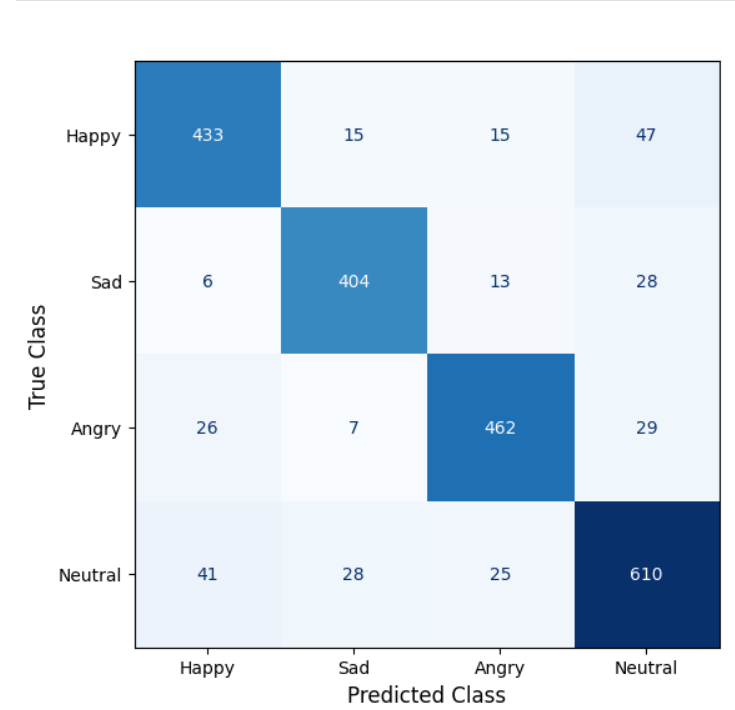
\includegraphics[width=1\linewidth]{cm}
	\caption{Confusion matrix of the \textsc{Daf-Cl} model.}
	\label{fig:cm}
\end{figure}

\begin{table}[ht]
	\centering
	\caption{\textsc{Daf-Cl} classification report.}
	\label{tab:report}
	
	\begin{tabular}{
			|>{\centering\arraybackslash}m{0.25\columnwidth}
			|>{\centering\arraybackslash}m{0.20\columnwidth}
			|>{\centering\arraybackslash}m{0.20\columnwidth}
			|>{\centering\arraybackslash}m{0.20\columnwidth}|
		}
		\hline
		\textbf{Classes} &
		\textbf{Precision \%} &
		\textbf{Recall \%} &
		\textbf{F1 Score \%} \\
		\hline
		\hline
		Happy & 85.43 & 86.65 & 86.04 \\
		\hline
		Sad & 89.71 & 88.71 & 88.93 \\
		\hline
		Angry & 88.99 & 89.58 & 89.28 \\
		\hline
		Neutral & 85.57 & 84.90 & 85.24 \\
		\hline
	\end{tabular}
\end{table}

\subsubsection{Comparison with Related Work}

To highlight the effectiveness of the proposed \textsc{Daf-Cl} framework, its performance was compared with recent multimodal emotion recognition methods that incorporate various contrastive learning strategies \cite{qian2022, Kim2023, Shi2024, Nguyen2024}, as reviewed in Section~\ref{sec:related work}. These studies were selected because they evaluate the same emotion classes considered by \textsc{Daf-Cl} and report results on the widely used IEMOCAP~\cite{Busso2008} and MELD~\cite{MELD2019} datasets. Tables~\ref{tab:Iemocap} and~\ref{tab:Meld} present the comparative results on the IEMOCAP and MELD datasets, respectively. Since the evaluation metrics reported by previous studies differ, the comparison is presented using the metrics available in the corresponding publications to ensure a fair and transparent evaluation.


\begin{table*}[ht]
	\centering
	\caption{Comparison of \textsc{Daf-Cl} with recent multimodal emotion recognition methods on the IEMOCAP dataset.}
	\label{tab:Iemocap}
	
	\begin{tabular}{
			|>{\centering\arraybackslash}m{0.8\columnwidth}
			|>{\centering\arraybackslash}m{0.2\columnwidth}
			|>{\centering\arraybackslash}m{0.2\columnwidth}
			|>{\centering\arraybackslash}m{0.2\columnwidth}|
		}
		\hline
		\textbf{Method} &
		\textbf{Weighted Accuracy (\%)} &
		\textbf{Unweighted Accuracy (\%)} &
		\textbf{Weighted F1 (\%)} \\
		\hline
		\hline
		Contrastive regularization for multimodal emotion recognition using audio and text \cite{qian2022} &
		76.06 &
		77.45 &
		-- \\
		\hline
		
		Enhancing emotion recognition in conversation through emotional coss-modal fusion and inter-class contrastive learning \cite{Shi2024} &
		68.77 &
		-- &
		68.66 \\
		\hline
		
		Focus-attention-enhanced crossmodal transformer with metric learning for multimodal speech emotion recognition \cite{Kim2023} &
		77.4 &
		77.7 &
		-- \\
		\hline
		
		
		HuBERT-CLAP: contrastive learning-based multimodal emotion recognition using self-alignment approach \cite{Nguyen2024} &
		77.22 &
		-- &
		-- \\
		\hline
		
		\textsc{\textbf{Daf-Cl} (Proposed)}: a robust multimodal emotion classification framework with dynamic adaptive fusion and contrastive learning &
		81.50 &
		82.92 &
		81.88 \\
		\hline
		
		\hline
	\end{tabular}
\end{table*}

\begin{table*}[ht]
	\centering
	\caption{Comparison of \textsc{Daf-Cl} with recent multimodal emotion recognition methods on the MELD dataset.}
	\label{tab:Meld}
	
	\begin{tabular}{
			|>{\centering\arraybackslash}m{0.8\columnwidth}
			|>{\centering\arraybackslash}m{0.2\columnwidth}
			|>{\centering\arraybackslash}m{0.2\columnwidth}
			|>{\centering\arraybackslash}m{0.2\columnwidth}|
		}
		\hline
		\textbf{Method} &
		\textbf{Accuracy (\%)} &
		\textbf{Weighted F1 (\%)} \\
		\hline
	
		Enhancing emotion recognition in conversation through emotional coss-modal fusion and inter-class contrastive learning \cite{Shi2024} &
		65.62 &
		64.73\\
		\hline
		
		\textsc{\textbf{Daf-Cl} (Proposed)}: a robust multimodal emotion classification framework with dynamic adaptive fusion and contrastive learning &
		81.66 &
		81.55 \\
		\hline
		
		\hline
	\end{tabular}
\end{table*}

As shown in Tables~\ref{tab:Iemocap} and~\ref{tab:Meld}, the proposed \textsc{Daf-Cl} framework consistently outperforms recent multimodal emotion recognition methods based on contrastive learning. On the IEMOCAP dataset, \textsc{Daf-Cl} achieves the highest performance across the reported evaluation metrics. Compared with the highest previously reported weighted accuracy of 77.40\%~\cite{Kim2023}, \textsc{Daf-Cl} improves the weighted accuracy by 4.10 percentage points. Similarly, the proposed framework improves the highest reported unweighted accuracy by 5.22 percentage points. These improvements demonstrate the effectiveness of combining dynamic adaptive fusion with contrastive learning to learn more discriminative multimodal representations.

A similar trend is observed on the MELD dataset, where \textsc{Daf-Cl} outperforms the most recent contrastive learning-based method by approximately 16 percentage points. The consistent improvements on both the acted IEMOCAP dataset and the conversational MELD dataset indicate that the proposed framework effectively exploits the complementary information provided by the acoustic and textual modalities, resulting in robust and generalizable multimodal emotion representations.
 

\subsubsection{Generalization to Unseen Datasets}
To further evaluate the robustness and generalization capability of \textsc{Daf-Cl}, the proposed model was evaluated on three completely unseen datasets: Emotional-EMA~\cite{ema}, EmoV-DB-sorted~\cite{emov}, and Emo-DB~\cite{emodb}. None of these datasets was used during training, and they contain different speakers and data distributions. Table~\ref{tab:unseen_results} summarizes the evaluated emotion classes, the number of recordings, and the corresponding F1 scores obtained by \textsc{Daf-Cl}. The results demonstrate that the proposed framework maintains consistently high performance across unseen datasets, indicating good generalization to previously unseen speakers and recording conditions.

Furthermore, the model achieved an F1 score of 90\% on the German Emo-DB dataset despite being trained primarily on English emotional speech corpora. This result suggests that the proposed framework exhibits a degree of cross-lingual generalization, although a more comprehensive evaluation on additional languages is required to fully assess its multilingual robustness.


\begin{table}[ht]
	\centering
	\caption{Generalization performance of \textsc{Daf-Cl} on unseen emotion recognition datasets.}
	\label{tab:unseen_results}
	
	\begin{tabular}{
			|>{\centering\arraybackslash}m{0.24\columnwidth}
			|>{\centering\arraybackslash}m{0.28\columnwidth}
			|>{\centering\arraybackslash}m{0.19\columnwidth}
			|>{\centering\arraybackslash}m{0.16\columnwidth}|
		}
		\hline
		\textbf{Dataset} &
		\textbf{Emotion Classes} &
		\textbf{Number of Recordings} &
		\textbf{F1 Score (\%)} \\
		\hline
		\hline
		Emotional-EMA &
		Happy, Sad, Angry, Neutral &
		680 &
		87 \\
		\hline
		
		EmoV-DB-sorted &
		Angry, Neutral &
		2,836 &
		93 \\
		\hline
		
		Emo-DB &
		Happy, Sad, Angry, Neutral &
		339 &
		90 \\
		\hline
	\end{tabular}
\end{table}



\subsection{Ablation Study}

To evaluate the contribution of each component in the proposed \textsc{Daf-Cl} framework, an ablation study was conducted by progressively extending a baseline model with the proposed modules while keeping all training settings unchanged. All experiments were performed on the same test set described in Section~\ref{subsec: data}, and performance was evaluated using the F1 score. This analysis quantifies the individual contribution of each module and demonstrates how the proposed components collectively improve the overall classification performance.

In addition to the progressive ablation study, several architectural design choices were investigated to justify the proposed implementation. Specifically, alternative variants of the chunk aggregation strategy, fusion strategy, layer adaptive weighting mechanism, and emotion similarity matrix were evaluated while keeping the remaining components unchanged. The results provide further insight into the impact of each design choice on the overall performance of \textsc{Daf-Cl}.

\subsubsection{Progressive Ablation Study}

The contribution of each component in the proposed \textsc{Daf-Cl} framework was evaluated through a progressive ablation study. Starting from a simplified multimodal baseline, one component was added at a time until the full proposed architecture was obtained. The baseline model uses the final hidden layer of WavLM instead of adaptive layer fusion, aggregates chunk-level audio representations using mean pooling, and combines the audio and text modalities through late fusion with a fixed weight of 0.5 for each modality. Both the cross-modal alignment loss and the structured supervised contrastive learning (SSCL) objective are excluded from the baseline.

Starting from this baseline, the following components were incrementally incorporated: (1) \textit{adaptive layer fusion}, which replaces the final WavLM hidden state with a learned weighted combination of multiple hidden layers; (2) \textit{chunk weighting}, which replaces uniform mean pooling with a learnable chunk aggregation strategy based on the gate $\alpha$ and classifier confidence; (3) \textit{dynamic fusion}, which replaces fixed modality weighting with an input-dependent fusion coefficient; (4) \textit{cross-modal alignment}, which introduces an alignment loss between utterance-level audio and text embeddings; and (5) \textit{SSCL}, which adds the proposed structured supervised contrastive learning objective using an emotion similarity matrix over audio chunk representations.

As shown in Table~\ref{tab:ablation}, adaptive layer fusion provides a clear improvement over the baseline, increasing the macro F1 score from 78.4\% to 82.3\%. This indicates that aggregating information from multiple WavLM layers is more effective than relying only on the final hidden layer. After adding chunk weighting, the macro F1 score slightly decreases to 81.4\%. This suggests that chunk-level weighting alone may not be sufficient when the audio embedding space is not yet well structured. However, when dynamic fusion is introduced, the performance increases to 82.9\%, indicating that input-dependent modality weighting helps the model adjust the contribution of audio and text according to the reliability of each utterance.

Adding cross-modal alignment further improves the macro F1 score to 84.8\%, demonstrating the benefit of reducing the representation gap between the audio and textual embedding spaces. Finally, incorporating SSCL leads to the best overall performance, achieving a macro F1 score of 87.4\%. This result shows that explicitly modeling structured relationships among emotion classes strengthens the discriminative quality of the learned audio representations. Overall, the full \textsc{Daf-Cl} framework improves the macro F1 score by 9.0 percentage points over the baseline, confirming that the proposed components are complementary and jointly contribute to the final performance.

\begin{table*}[ht]
	\centering
	\caption{Progressive ablation study of the proposed \textsc{Daf-Cl} framework. Each model variant incrementally incorporates one additional component while keeping all other training settings unchanged.}
	\label{tab:ablation}
	\begin{tabular}{
			|l|
			>{\centering\arraybackslash}m{0.16\columnwidth}|
			>{\centering\arraybackslash}m{0.16\columnwidth}|
			>{\centering\arraybackslash}m{0.16\columnwidth}|
			>{\centering\arraybackslash}m{0.18\columnwidth}|
			>{\centering\arraybackslash}m{0.18\columnwidth}|
			>{\centering\arraybackslash}m{0.14\columnwidth}|
		}
		\hline
		\textbf{Model Variant} &
		\textbf{Adaptive Layer Fusion} &
		\textbf{Chunk Weighting} &
		\textbf{Dynamic Fusion} &
		\textbf{Cross-modal Alignment} &
		\textbf{SSCL} &
		\textbf{Macro F1 (\%)} \\
		\hline
		Baseline &
		-- & -- & -- & -- & -- &
		78.4 \\
		\hline
		+ Adaptive Layer Fusion &
		$\checkmark$ & -- & -- & -- & -- &
		82.3 \\
		\hline
		+ Chunk Weighting &
		$\checkmark$ & $\checkmark$ & -- & -- & -- &
		81.4 \\
		\hline
		+ Dynamic Fusion &
		$\checkmark$ & $\checkmark$ & $\checkmark$ & -- & -- &
		82.9 \\
		\hline
		+ Cross-modal Alignment &
		$\checkmark$ & $\checkmark$ & $\checkmark$ & $\checkmark$ & -- &
		84.8 \\
		\hline
		+ SSCL (Proposed) &
		$\checkmark$ & $\checkmark$ & $\checkmark$ & $\checkmark$ & $\checkmark$ &
		\textbf{87.4} \\
		\hline
	\end{tabular}
\end{table*}


\subsubsection{Impact of the Chunk Aggregation Strategy} \label{subsec: chunk}
To justify our chunk aggregation design choice, we evaluate five alternative strategies for combining chunk-level predictions into an utterance-level representation, under an otherwise identical training configuration. For the mean pooling, max pooling, and confidence-only variants, audio and text logits are combined using a fixed, equally weighted fusion (0.5 for each modality), since these variants do not produce a learned per-utterance gate for dynamic fusion. Table~\ref{tab:chunkimpact} reports the resulting macro F1 scores.

As shown, simple pooling strategies (mean and max) yield the weakest performance, since they treat all chunks as equally informative regardless of their acoustic content or the classifier's certainty about them. The learned gate ($\alpha$ only) improves modestly over pooling, but its capacity is limited: $\alpha$ is learned solely from the chunk's acoustic embedding and has no access to how the classifier is currently behaving on that chunk, making it prone to relying on superficial acoustic cues rather than a reliable indicator of chunk informativeness. Confidence-only weighting performs better still, as it is derived directly from the classifier's own output entropy and therefore adapts to the model's evolving decision boundary; however, it cannot by itself distinguish genuinely informative chunks from chunks on which the classifier is confidently wrong. Combining the two signals ($\text{confidence} \times \alpha$) consistently yields the best performance, as the two mechanisms compensate for each other's weaknesses: a chunk receives high weight only when it is both acoustically salient (high $\alpha$) and one on which the classifier currently expresses low uncertainty (high confidence), effectively penalizing chunks that would otherwise mislead the final prediction. This joint criterion proves more robust than either signal in isolation.

\begin{table}[ht]
	\centering
	\caption{Impact of chunk aggregation strategy on macro F1 score.}
	\label{tab:chunkimpact}
	\begin{tabular}{
			|l|
			>{\centering\arraybackslash}m{0.30\columnwidth}|
		}
		\hline
		\textbf{Chunk Aggregation Method} &
		\textbf{Macro F1 (\%)} \\
		\hline
		Mean pooling &
		83.1  \\
		\hline
		Max pooling &
		82.9 \\
		\hline
		Learned $\alpha$ only &
		83.4 \\
		\hline
		Confidence only &
		84.1 \\
		\hline
		Confidence $\times$ $\alpha$ (proposed) &
		\textbf{87.4} \\
		\hline
	\end{tabular}
\end{table}

\subsubsection{Impact of the Fusion Strategy}

To evaluate the effectiveness of the proposed fusion strategy, four multimodal fusion approaches were compared: (1) \textit{early fusion}, where the audio and text embeddings are concatenated at the feature level and processed by a shared classification head; (2) \textit{late fusion with equal weighting}, where each modality is classified independently and the predicted logits are combined using a fixed weight of 0.5 for each modality; (3) \textit{late fusion with a dedicated learnable gate}, where a separate gating network jointly processes the audio and text embeddings to estimate the fusion weight; and (4) the proposed \textit{dynamic fusion} strategy in \textsc{Daf-Cl}, which also performs late fusion with a learnable gate but reuses the weighting coefficient, $\alpha$, learned during chunk aggregation instead of introducing an additional cross-modal gating network. Unlike the dedicated learnable gate, which must learn the relative importance of the two modalities from scratch, the proposed approach reuses the weighting coefficient learned during chunk aggregation, which provides a reliability-aware signal for the acoustic representation.

Table \ref{tab:fusionimpact} presents the macro F1 scores obtained using each fusion strategy. Early fusion achieves the lowest performance in this experimental setting, suggesting that directly concatenating the audio and textual representations may not be sufficient to fully exploit their complementary information within the proposed framework. Late fusion with equal weighting improves the classification performance in this setting, suggesting that allowing each modality to make an independent prediction before combining their outputs is more effective than direct feature-level concatenation for the evaluated task. This suggests that learning an additional cross-modal gating function may increase the optimization difficulty and reduce generalization under the available training data. In contrast, the proposed dynamic fusion strategy achieves the highest macro F1 score. By reusing the chunk-level weighting coefficient as the fusion weight, the proposed framework avoids introducing an additional gating network while exploiting a reliability-aware signal learned during chunk aggregation. This leads to a more stable and effective multimodal fusion mechanism, as reflected by the highest macro F1 score in Table~\ref{tab:fusionimpact}.

\begin{table}[ht]
	\centering
	\caption{Impact of different fusion strategies on macro F1 score.}
	\label{tab:fusionimpact}
	\begin{tabular}{
			|l|
			>{\centering\arraybackslash}m{0.30\columnwidth}|
		}
		\hline
		\textbf{Fusion Strategy} &
		\textbf{Macro F1 (\%)} \\
		\hline
		Early fusion &
		83.7 \\
		\hline
		Late fusion with equal weighting &
		85.7 \\
		\hline
		Late fusion with dedicated learnable gate &
		85.0 \\
		\hline
		Proposed dynamic fusion &
		\textbf{87.4} \\
		\hline
	\end{tabular}
\end{table}

\subsubsection{Impact of the Layer Aggregation Strategy}

To justify our choice of layer aggregation strategy, we compare three variants for combining the $L$ hidden layers produced by the audio encoder: (1) using only the \textit{last hidden layer}, a common choice in prior speech emotion recognition literature; (2) \textit{averaging all hidden layers} uniformly; and (3) our proposed \textsc{Daf-Cl} \textit{adaptive layer weighting}, which learns a softmax-normalized weight for each layer and combines them via a weighted sum, allowing the model to determine the contribution of each layer directly from the training data.

Table~\ref{tab:layerimpact} reports the macro F1 score for each variant. Under our training setting, incorporating information from all layers substantially outperforms relying on the last layer alone, indicating that emotion-relevant information is distributed across the encoder's depth rather than concentrated solely in its final representation. The proposed adaptive weighting further improves over uniform averaging, showing that allowing the model to learn a layer-specific weighting, rather than treating all layers as equally informative, provides a consistent advantage.

\begin{table}[ht]
	\centering
	\caption{Impact of layer aggregation strategy on macro F1 score.}
	\label{tab:layerimpact}
	\begin{tabular}{
			|l|
			>{\centering\arraybackslash}m{0.30\columnwidth}|
		}
		\hline
		\textbf{Layer Representation} &
		\textbf{Macro F1 (\%)} \\
		\hline
		Last hidden layer &
		82.30  \\
		\hline
		Average all layers &
		86.50 \\
		\hline
		Proposed adaptive weighting &
		87.40 \\
		\hline
	\end{tabular}
\end{table}

To better understand what the adaptive weighting mechanism learns, we inspect the softmax-normalized layer weights $\text{softmax}(\mathbf{w})$ from the trained model, shown in Figure~\ref{fig:layerweights}. The learned weights assign a mild but consistent preference to the upper-middle layers of the encoder, peaking at layer 10 (weight $= 0.103$), while the earliest layers (1--7) and the final layer (12) receive weights slightly below the uniform baseline ($1/L = 0.083$). Notably, no single layer dominates the aggregation: all weights remain within a narrow range (0.074--0.103), indicating that the model retains and combines information from nearly all layers rather than collapsing onto a small subset. This suggests that the performance gain from adaptive weighting stems from a mild, learned redistribution of emphasis across layers rather than from discarding most of the encoder's depth, which is consistent with the observation that averaging all layers already performs close to the proposed method (Table~\ref{tab:layerimpact}). The relatively lower weight assigned to the final layer is consistent with prior findings that the last layers of self-supervised speech encoders tend to specialize toward the pretraining objective rather than downstream paralinguistic tasks \cite{pepino21_interspeech}, making upper-middle layers a more informative source for emotion-discriminative features in this setting.

\begin{figure}[ht]
	\centering
	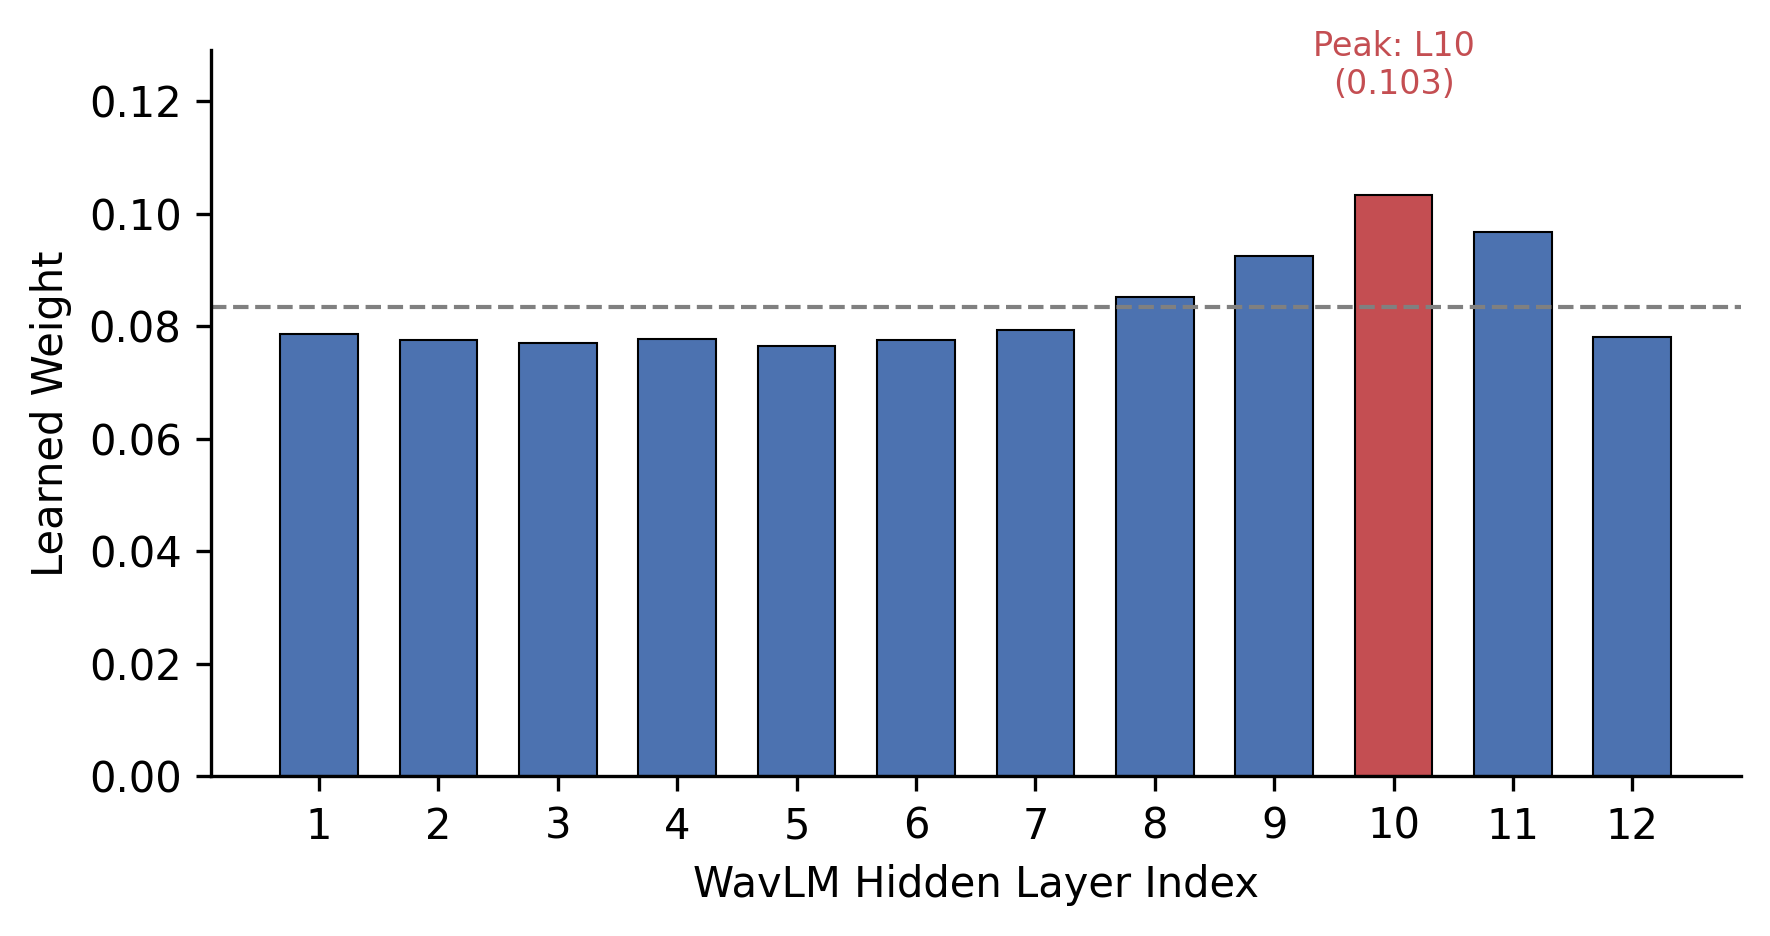
\includegraphics[width=0.85\columnwidth]{layer_weights.png}
	\caption{Learned adaptive layer weights (softmax-normalized) across the 12 WavLM hidden layers. The dashed line marks the uniform weight ($1/L$) for reference; layers above it contribute more to the fused representation than a simple average would assign, while layers below it contribute less.}
	\label{fig:layerweights}
\end{figure}

\subsubsection{Impact of the Emotion Similarity Matrix} 

To evaluate the contribution of the proposed emotion similarity matrix, we compare the structure supervised contrastive loss (SSCL) with the standard supervised contrastive loss (SupCon)~\cite{khosla2020supervised}. In standard SupCon, samples from the same class are treated as positive pairs, whereas samples from different classes are treated as negative pairs. This hard positive/negative formulation ignores the graded relationships that may exist between emotion classes. In contrast, the proposed formulation incorporates an emotion similarity matrix into the contrastive objective to model soft inter-class relationships.

It should be emphasized that the proposed similarity matrix is used only within the contrastive learning objective to regularize the learned audio embedding space; it does not modify the ground-truth labels or the final classification objective. Thus, the classifier is still optimized to distinguish the target emotion categories, while the contrastive objective encourages the audio representation to preserve meaningful similarities among emotionally related classes. This is particularly relevant for speech emotion recognition, where emotions may overlap acoustically and perceptually rather than forming completely independent clusters.

As shown in Table~\ref{tab:emotionimpact}, incorporating the proposed emotion similarity matrix improves the macro F1 score compared with standard SupCon. This result suggests that preserving soft relationships among emotion classes provides a more informative supervision signal than treating all different-class pairs as equally dissimilar. By encoding these graded relationships, the proposed contrastive objective learns a more structured audio embedding space, which contributes to improved classification performance.

\begin{table}[ht]
	\centering
	\caption{Impact of the proposed emotion similarity matrix on macro F1 score.}
	\label{tab:emotionimpact}
	\begin{tabular}{
			|l|
			>{\centering\arraybackslash}m{0.30\columnwidth}|
		}
		\hline
		\textbf{SupCon Variant} &
		\textbf{Macro F1 (\%)} \\
		\hline
		Standard SupCon &
		86.20 \\
		\hline
		Proposed emotion similarity matrix &
		\textbf{87.40} \\
		\hline
	\end{tabular}
\end{table}


\subsection{Sensitivity Analysis}

To examine the robustness of \textsc{Daf-Cl} with respect to its main hyperparameters, a sensitivity analysis was conducted on the parameters that directly affect the proposed components. Specifically, we investigated the loss weighting coefficients $\lambda_{\text{align}}$ and $\lambda_{\text{SSCL}}$, which control the contribution of the cross-modal alignment loss and the structured supervised contrastive learning objective, respectively. In addition, the temperature parameter $\tau$ and the audio segmentation parameters, including chunk size and chunk overlap, were evaluated. Unless otherwise stated, all experiments were conducted under the same training and evaluation settings, and performance was measured using macro F1 score.

\subsubsection{Sensitivity to $\lambda_{\text{align}}$}

The coefficient $\lambda_{\text{align}}$ controls the contribution of the cross-modal alignment loss during training. This loss encourages the audio and textual representations of the same utterance to be closer in the shared embedding space. However, an excessively small value may limit the effect of alignment, whereas an overly large value may dominate the main classification objective. Therefore, different values of $\lambda_{\text{align}}$ were evaluated to identify a suitable balance between classification learning and cross-modal representation alignment.

As shown in Table \ref{tab:lambda_align}, the best macro F1 score is achieved when $\lambda_{\text{align}}=0.4$, which corresponds to the setting used in the proposed \textsc{Daf-Cl} framework. A smaller value, such as $\lambda_{\text{align}}=0.1$, results in lower performance, suggesting that weak alignment is insufficient to effectively reduce the gap between the audio and textual embedding spaces. Increasing the coefficient to 0.2 improves the performance, confirming the benefit of incorporating the alignment loss. However, further increasing the value to 0.6 slightly reduces the macro F1 score, indicating that assigning excessive weight to the alignment objective may negatively affect the discriminative learning required for emotion classification. These results suggest that $\lambda_{\text{align}}=0.4$ provides an effective trade-off between cross-modal alignment and classification performance.

\begin{table}[ht]
	\centering
	\caption{Sensitivity analysis of the cross-modal alignment loss coefficient $\lambda_{\text{align}}$.}
	\label{tab:lambda_align}
	\begin{tabular}{
			|>{\centering\arraybackslash}m{0.35\columnwidth}|
			>{\centering\arraybackslash}m{0.35\columnwidth}|
		}
		\hline
		\textbf{$\lambda_{\text{align}}$} &
		\textbf{Macro F1 (\%)} \\
		\hline
		0.1 & 84.42 \\
		\hline
		0.2 & 85.3 \\
		\hline
		0.4 & \textbf{87.40} \\
		\hline
		0.6 & 86.1 \\
		\hline
	\end{tabular}
\end{table}



\subsubsection{Sensitivity to $\lambda_{\text{SSCL}}$}

The coefficient $\lambda_{\text{SSCL}}$ controls the contribution of the structured supervised contrastive learning objective during training. This objective regularizes the learned audio representation by encouraging better separation between emotion classes while preserving the structured relationships defined by the emotion similarity matrix. However, assigning an insufficient weight may limit the effect of contrastive learning, whereas an excessively large value may overemphasize the auxiliary representation-learning objective at the expense of the main classification objective. Therefore, different values of $\lambda_{\text{SSCL}}$ were evaluated to identify an appropriate balance.

As shown in Table \ref{tab:lambda_sscl}, the best macro F1 score is obtained when $\lambda_{\text{SSCL}}=0.3$, which is the value adopted in the proposed \textsc{Daf-Cl} framework. A lower value, such as $\lambda_{\text{SSCL}}=0.1$, results in comparatively lower performance, suggesting that weak contrastive supervision may be insufficient to learn highly discriminative emotion representations. Increasing the coefficient to 0.2 improves the macro F1 score, confirming the benefit of the SSCL objective. However, further increasing the value to 0.5 slightly decreases performance, indicating that excessive emphasis on the auxiliary contrastive objective may reduce the model's ability to optimize the final classification task. Although $\lambda_{\text{SSCL}}=0.3$ yields the highest macro F1 score, the performance remains relatively stable across the evaluated range. This indicates that the SSCL objective consistently contributes to representation learning, while the selected value provides the best balance between enhancing emotion-class separability and preserving the optimization of the main classification objective.

\begin{table}[ht]
	\centering
	\caption{Sensitivity analysis of the structured supervised contrastive learning coefficient $\lambda_{\text{SSCL}}$.}
	\label{tab:lambda_sscl}
	\begin{tabular}{
			|>{\centering\arraybackslash}m{0.35\columnwidth}|
			>{\centering\arraybackslash}m{0.35\columnwidth}|
		}
		\hline
		\textbf{$\lambda_{\text{SSCL}}$} &
		\textbf{Macro F1 (\%)} \\
		\hline
		0.1 & 85.81 \\
		\hline
		0.2 & 86.15 \\
		\hline
		0.3 & \textbf{87.40} \\
		\hline
		0.5 & 86.65 \\
		\hline
	\end{tabular}
\end{table}


\subsubsection{Sensitivity to the Temperature Parameter $\tau$}

The temperature parameter $\tau$ controls the sharpness of the similarity distribution in the contrastive learning objective. A smaller value of $\tau$ increases the emphasis on hard positive and negative pairs, leading to stronger separation in the embedding space. In contrast, a larger value produces a smoother similarity distribution, which may reduce the discriminative effect of the contrastive objective. Following common settings in contrastive learning, values in the range of 0.05 to 0.2 were evaluated.

As shown in Table \ref{tab:tau_sensitivity}, the best macro F1 score is achieved when $\tau=0.07$, which is the value adopted in the proposed \textsc{Daf-Cl} framework. Reducing the temperature to 0.05 slightly decreases performance, suggesting that excessive sharpening of the similarity distribution may overemphasize difficult pairs. Increasing $\tau$ to 0.1 and 0.2 leads to a larger performance reduction, indicating that a smoother similarity distribution weakens the ability of the contrastive objective to learn sufficiently discriminative emotion representations. These results show that $\tau=0.07$ provides the most effective balance between hard-pair emphasis and stable representation learning.

\begin{table}[ht]
	\centering
	\caption{Sensitivity analysis of the temperature parameter $\tau$.}
	\label{tab:tau_sensitivity}
	\begin{tabular}{
			|>{\centering\arraybackslash}m{0.35\columnwidth}|
			>{\centering\arraybackslash}m{0.35\columnwidth}|
		}
		\hline
		\textbf{$\tau$} &
		\textbf{Macro F1 (\%)} \\
		\hline
		0.05 & 86.19 \\
		\hline
		0.07 & \textbf{87.40} \\
		\hline
		0.10 & 85.55 \\
		\hline
		0.20 & 85.00 \\
		\hline
	\end{tabular}
\end{table}


\subsubsection{Sensitivity to Chunk Size}

The proposed \textsc{Daf-Cl} framework segments each audio utterance into fixed-length chunks to capture local emotional cues while supporting the processing of longer recordings. The chunk representations are subsequently aggregated to obtain an utterance-level acoustic representation. Considering the duration distribution of the training data, where the average utterance length is approximately 3~s, three chunk sizes of 2, 3, and 4~s were evaluated to examine the trade-off between temporal resolution and contextual coverage.

As shown in Table~\ref{tab:chunk_sensitivity}, the performance remains relatively stable across the evaluated chunk sizes, indicating that \textsc{Daf-Cl} is not highly sensitive to moderate variations in this parameter. A chunk size of 3~s achieves the highest macro F1 score of 87.40\% and is therefore adopted in the proposed framework. Shorter 2~s chunks provide finer temporal resolution but may capture less contextual information, whereas longer 4~s chunks provide broader context at the cost of reduced temporal granularity. The results suggest that a 3~s chunk size provides an appropriate balance between local emotional information and utterance-level context for the evaluated data.

\begin{table}[ht]
	\centering
	\caption{Sensitivity analysis of the audio chunk size.}
	\label{tab:chunk_sensitivity}
	\begin{tabular}{
			|>{\centering\arraybackslash}m{0.35\columnwidth}|
			>{\centering\arraybackslash}m{0.35\columnwidth}|
		}
		\hline
		\textbf{Chunk Size (s)} &
		\textbf{Macro F1 (\%)} \\
		\hline
		2 & 86.27 \\
		\hline
		3 & \textbf{87.40} \\
		\hline
		4 & 86.68 \\
		\hline
	\end{tabular}
\end{table}



\subsubsection{Sensitivity to Chunk Overlap}

To reduce the risk of losing emotionally relevant information at chunk boundaries, adjacent audio segments were processed with temporal overlap. Increasing the overlap provides greater continuity between neighboring chunks and allows transitional acoustic cues to be captured by more than one segment. However, excessive overlap also increases redundancy and computational cost. Therefore, overlap ratios of 0.25, 0.50, and 0.75 were evaluated to examine the trade-off between classification performance and processing efficiency.

As shown in Table~\ref{tab:chunk_overlap}, the lowest overlap ratio of 0.25 results in a lower macro F1 score, suggesting that limited overlap may omit useful contextual information around chunk boundaries. Increasing the overlap to 0.50 substantially improves performance, while a further increase to 0.75 does not provide an additional benefit and yields a comparable macro F1 score. Based on this result, an overlap ratio of 0.50 is adopted in the proposed \textsc{Daf-Cl} framework, as it provides the best observed performance while avoiding the additional redundancy and computational overhead associated with a larger overlap.

\begin{table}[ht]
	\centering
	\caption{Sensitivity analysis of the audio chunk overlap ratio.}
	\label{tab:chunk_overlap}
	\begin{tabular}{
			|>{\centering\arraybackslash}m{0.35\columnwidth}|
			>{\centering\arraybackslash}m{0.35\columnwidth}|
		}
		\hline
		\textbf{Chunk Overlap} &
		\textbf{Macro F1 (\%)} \\
		\hline
		0.25 & 85.10 \\
		\hline
		0.50 & \textbf{87.40} \\
		\hline
		0.75 & 87.00 \\
		\hline
	\end{tabular}
\end{table}


\subsection{Representation Analysis}

To qualitatively investigate the effect of the proposed structured supervised contrastive learning (SSCL) objective on the learned audio representation space, t-SNE was applied to the chunk-level audio embeddings obtained before and after incorporating SSCL. A balanced subset of 1,000 embeddings was randomly selected from the evaluation set, comprising 250 samples from each emotion class. The same samples and t-SNE configuration were used for both models to enable a consistent visual comparison.

Figure~\ref{fig:tsne_sscl} illustrates the resulting two-dimensional embedding distributions. Without SSCL, substantial overlap can be observed among the emotion classes, indicating limited structure in the learned audio representation space. After incorporating SSCL, the embeddings exhibit more compact within-class distributions and more distinguishable inter-class organization. Nevertheless, some overlap remains, particularly between the \textit{happy} and \textit{neutral} classes. This pattern is consistent with the classification results, where these two classes exhibit greater confusion and comparatively lower class-level performance than the other emotion categories.

The observed change in the embedding distribution provides qualitative support for the role of SSCL in organizing the audio representation space. In particular, the structured contrastive objective encourages discriminative class representations while preserving graded relationships among emotionally similar classes through the proposed emotion similarity matrix. This observation is also consistent with the performance improvements reported in the ablation study. Since t-SNE is a nonlinear dimensionality-reduction technique and does not directly quantify class separability, the visualization is used as complementary qualitative evidence rather than as an independent measure of representation quality.

\begin{figure*}[ht]
	\centering
	\begin{tabular}{cc}
		\includegraphics[width=0.85\columnwidth]{"tsne_without_sscl (1)"} & 
		\includegraphics[width=0.85\columnwidth]{"tsne_with_sscl (1)"} \\
		\small{(a) Without SSCL} &
		\small{(b) With SSCL}
	\end{tabular}
	\caption{t-SNE visualization of the chunk-level audio embedding space without and with the proposed SSCL objective. The same balanced subset of 1,000 embeddings (250 per emotion class) is used in both visualizations.}
	\label{fig:tsne_sscl}
\end{figure*}



\section{Limitations and Future Work}\label{sec: limitations}

\input{Limitations & Future Work }

\section{Conclusions}\label{sec:Conclusion}

\input{conclusion}




\bibliography{references}
\bibliographystyle{IEEEtran}

% \begin{IEEEbiographynophoto}{Saja R. Taweel} received her Bachelor's degree in Data Science and Artificial Intelligence from Princess Sumaya University for Technology, Amman, Jordan, in 2024. Her current research focuses on optimizing resource allocation and management in hospitals during pandemics. She is particularly interested in applying machine learning and predictive analytics to solve real-world challenges. 
% \end{IEEEbiographynophoto}

% \begin{IEEEbiography}


% \end{IEEEbiography}





\end{document}
